\chapter{PX4 autopilot}

PX4 je profesionální autopilot, vyvinutý světovými vývojáři z průmyslu a akademické obce a podporovaný aktivní celosvětovou komunitou. Pohání všechny druhy vozidel od závodních a nákladních dronů až po pozemní vozidla a ponorky. 

\section{QGround Control}

QGroundControl je software, který poskytuje plnou kontrolu letu a plánování mise pro jakýkoli dron s podporou MAVLink. Jeho primárním cílem je snadné použití pro profesionální uživatele a vývojáře. Veškerý kód je open source, takže je možné přispívat a dál ho vyvíjet \cite{QGround}.
TODO nejaké screenshoty z aplikácie

\subsection{Nastavení vozidel}

\subsubsection{Podporované typy vozidel}

\subsection{Plánování bezpilotní mise}


\section{Licence}

Kód PX4 je zdarma k použití a úpravě za podmínek permisivní licence \textit{BSD 3-clause license} \cite{BSDlicense}.

Redistribuce a použití ve zdrojové a binární formě, s úpravami nebo bez nich, jsou povoleny za předpokladu, že jsou splněny následující podmínky:

1. Redistribuce zdrojového kódu musí obsahovat výše uvedenou poznámku o autorských právech, tento seznam podmínek a následující prohlášení o vyloučení odpovědnosti.

2. Redistribuce v binární formě musí reprodukovat výše uvedenou poznámku o autorských právech, tento seznam podmínek a následující prohlášení o vyloučení odpovědnosti v dokumentaci a/nebo jiných materiálech dodávaných s distribucí.

3. Jméno držitele autorských práv ani jména jeho přispěvatelů nesmí být použita k podpoře nebo propagaci produktů odvozených z tohoto software bez předchozího výslovného písemného povolení.

\section{Vnitřní struktura PX4}

\section{Přepojení s simulátorem Gazebo}

\subsection{Komunikace}

\section{Přepojení PX4 s ROS2}

\subsection{ROS2 aplikace}

\subsection{ROS2 zprávy}

\subsection{MicroRTPS agent a klient}


\section{DDS/RTPS middleware}

Služba OMG\footnote{Object Management Group\textsuperscript \textregistered (OMG\textsuperscript \textregistered) je mezinárodní neziskové konsorcium pro technologické standardy s otevřeným členstvím.} Data-Distribution Service for Real-Time Systems\textsuperscript \textregistered (\acs{DDS}) je prvním otevřeným mezinárodním middlewarovým standardem, který přímo řeší komunikaci pro \textit{publish and subscribe} systémy v reálném čase.

\acs{DDS} představuje virtuální globální datový prostor, kde mohou aplikace sdílet informace pouhým čtením a zápisem datových objektů. Datové objekty jsou adresované pomocí definovaného názvu (\textit{topic}) a klíče (\textit{key}). \acs{DDS} integruje součásti systému dohromady a poskytuje datovou konektivitu s nízkou latencí, extrémní spolehlivost a škálovatelnou architekturu. Nabízí rozsáhlé řízení parametrů \acs{QoS} (\acl{QoS}), včetně spolehlivosti, šířky pásma a limitů zdrojů \cite{DDS_Def}. 

\acs{DDS} middleware komunikuje peer-to-peer a nevyžaduje, aby byla data zprostředkována serverem nebo cloudem. 

Jak je zobrazeno na obr \ref{fig:DDSmiddleware}, \acs{DDS} middleware je software vrstva, která odděluje aplikaci od detailů operačního systému, síťového přenosu a nízkoúrovňových datových formátů. Nízkoúrovňové detaily, jako je formát dat v paměti, spolehlivost, protokoly, výběr přenosového kanálu, \acs{QoS}, zabezpečení atd. jsou spravovány middlewarem. 

\begin{figure}[!ht]
  \begin{center}
    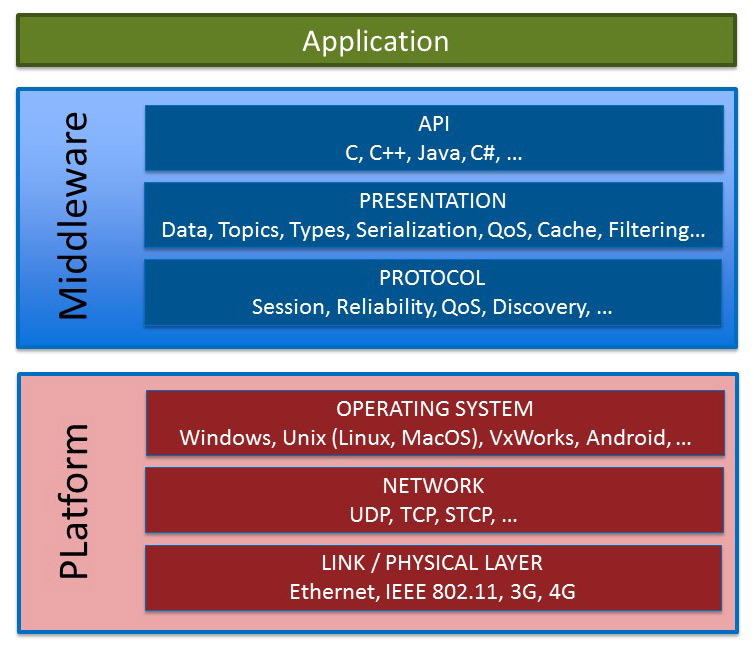
\includegraphics[scale=0.4]{obrazky/DDS1}
  \end{center}
  \caption[Propojení \acs{DDS} middlewaru s aplikací a operačním systémem]{Propojení \acs{DDS} middlewaru s aplikací a operačním systémem \cite{DDS_Main}.}
  \label{fig:DDSmiddleware}
\end{figure}

\subsection{\acs{DDS} a ROS 2}

\acs{DDS} middleware je základní komunikační interface pro ROS 2. Middleware zajišťuje dynamické hledání bodů v síti, serializaci a \textit{publish/subscribe} přenos dat. ROS 2 skrývá velkou část složitosti \acs{DDS} pro většinu uživatelů, ale taky poskytuje přístup k základní implementaci \acs{DDS} pro uživatele, kteří potřebují vyřešit extrémní případy nebo potřebují integraci s jinými stávající \acs{DDS} systémy. \cite{ROS2DDS}

ROS 2 podporuje více implementací \acs{DDS}/RTPS. Při výběru implementace middlewaru můžete zvážit mnoho faktorů, jako je licence, dostupnost platformy nebo výpočetní náročnost. Existují varianty middleware, které jsou vytvořeny pro mikrokontroléry, nebo varianty, které se zaměřují na aplikace vyžadující speciální bezpečnostní certifikace.

Podpora několika implementací \acs{DDS} middleware je důležitá pro zajištění toho, aby kódová základna ROS 2 nebyla vázána na žádnou konkrétní implementaci, protože uživatelé mohou chtít implementace přepínat v závislosti na potřebě jejich projektu. \cite{ROS2DDS2}

ROS 2 podporuje tyto \acs{DDS} implementace:
\begin{itemize}
    \item RTI (Real-Time Innovations) Connext
    \item Eclipse Cyclone DDS
    \item eProsima Fast DDS
\end{itemize}

\subsection{Orientace na data (data centricity)}

\acs{DDS} middleware je jeden z mála middleware, který je zaměřen na data. Orientace na data zajišťuje, že všechny zprávy obsahují správné kontextové informace, které aplikace potřebuje k pochopení dat, která přijímají.

Podstatou orientace na data je, že \acs{DDS} middleware má informaci o tom, jaká data ukládá, a řídí, jak tato data sdílet. Programátoři používající tradiční middleware zaměřený na zprávy musí napsat kód, který odesílá zprávy. Programátoři používající middleware orientovaný na data píší kód, který určuje, jak a kdy sdílet data a poté přímo sdílejí datové hodnoty. \acs{DDS} přímo implementuje řízené, spravované a bezpečné sdílení dat. \cite{DDS_Main}

\subsection{Globální datový prostor}

\acs{DDS} aplikace má přístup k lokálnímu úložišti dat nazývanému \textit{globální datový prostor}. \textit{Globální datový prostor} vypadá pro aplikaci jako lokální paměť přístupná přes \acs{API} (\acl{API}). \acs{DDS} middleware posílá zprávy k aktualizaci příslušných úložišť na vzdálených komunikačních uzlech (\textit{nodes}).

V \acs{DDS} aplikacích neexistuje žádné globální datové místo, kde by všechna data existovala. Každá aplikace si lokálně ukládá jen to, co potřebuje a jen tak dlouho, jak to potřebuje. \cite{DDS_Main}

\acs{DDS} se zabývá daty v pohybu - globální datový prostor je virtuální koncept, který je ve skutečnosti pouze souborem lokálních úložišť. Každá aplikace, téměř v jakémkoli jazyce, běžící na jakémkoli systému, vidí lokální paměť ve svém optimálním nativním formátu. Globální datový prostor sdílí data mezi vestavěnými, mobilními a cloudovými aplikacemi v rámci jakéhokoli přenosu, bez ohledu na jazyk nebo systém, a s extrémně nízkou latencí.

\subsection{Základní architektura \acs{DDS}}

Nejzákladnějším komunikačním vzorem podporovaným \acs{DDS} je model publikování/přihlášení (\textit{Publish/Subscribe}). \textit{Publish/Subscribe} je komunikační model, kde producenti dat publikují data a spotřebitelé dat se přihlašují k odběru dat. Tito producenti a spotřebitelé o sobě nemusí vědět předem, protože se navzájem dynamicky objevují za běhu. Data, která sdílejí, jsou popsána tématem (\textit{topic}) a producenti a spotřebitelé odesílají a přijímají data pouze pro témata, která je zajímají. V tomto vzoru může mnoho producentů publikovat stejné téma a mnoho spotřebitelů se může přihlásit k odběru stejného tématu. Spotřebitelé dostávají data od všech producentů, se kterými sdílejí téma. Producenti odesílají data přímo Spotřebitelům, aniž by potřebovali brokera nebo centralizovanou aplikaci pro zprostředkování komunikace. \cite{DDS_PubSub}

Jak je zobrazeno na obrázku \ref{fig:DDSarch} v \acs{DDS} se objekty, které publikují data, nazývají \textit{DataWriters} a objekty, které odebírají data, jsou \textit{DataReaders}. \textit{DataWriters} a \textit{DataReaders} jsou spojeni s jedním objektem \textit{Topic}, který tato data popisuje.

\begin{figure}[!ht]
  \begin{center}
    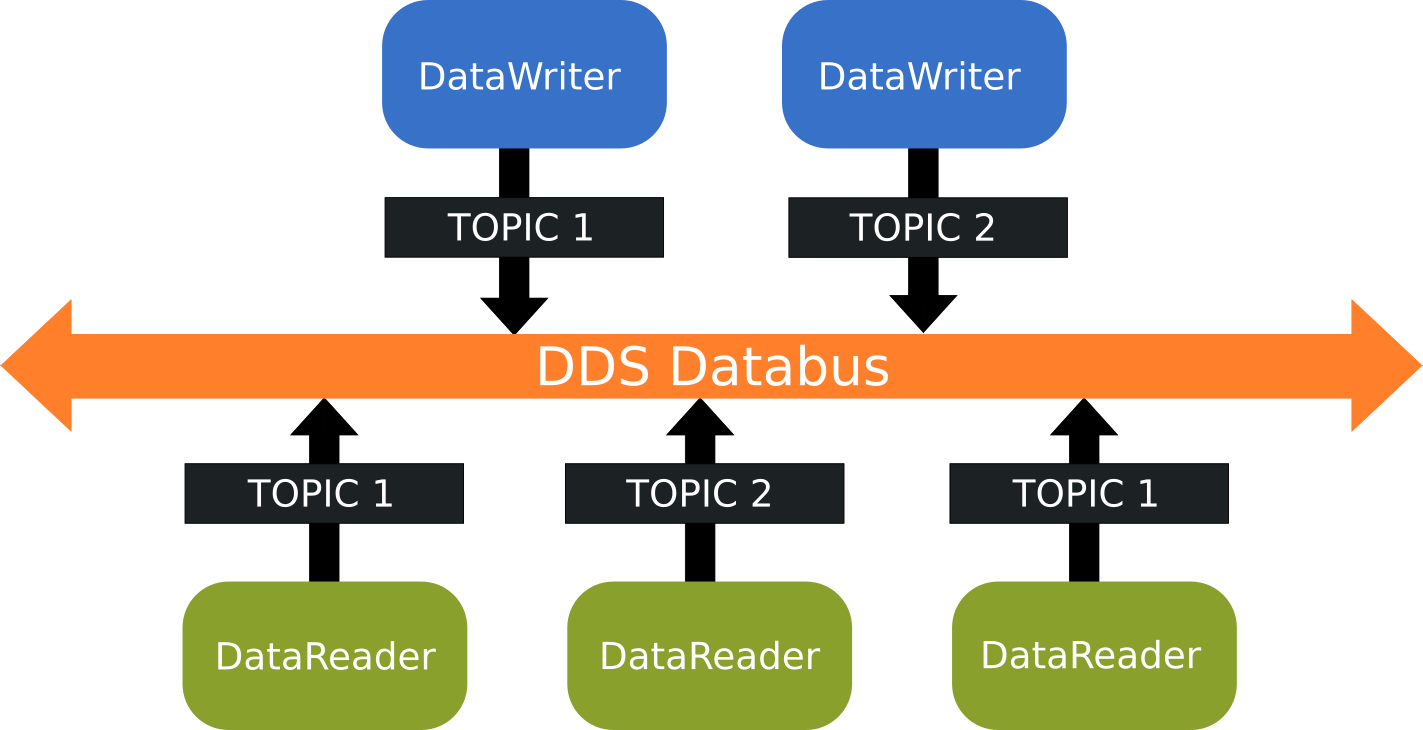
\includegraphics[scale=0.35]{obrazky/DDS2}
  \end{center}
  \caption[Základní \textit{publish/subscribe} struktura \acs{DDS} komunikace]{Základní \textit{publish/subscribe} struktura \acs{DDS} komunikace \cite{DDS_PubSub}.}
  \label{fig:DDSarch}
\end{figure}

\subsection{Quality of Service}

V \acs{DDS} aplikacích je možné sdílet data s flexibilními specifikacemi kvality služeb (\acs{QoS}), jako jsou spolehlivost, stav systému, živost, zabezpečení a mnohé další. 

\acs{DDS} middleware posílá jen data, které jsou nutné pro správnou funkci systému. Pokud se zprávy nedostanou do zamýšlených cílů, middleware automaticky zvýší spolehlivost na daných datových cestách. Když se komunikační systémy změní, middleware dynamicky zjistí, kam poslat data, a informuje účastníky o změnách. Pokud je celková velikost dat obrovská, \acs{DDS} inteligentně filtruje a odesílá pouze data, která každý koncový bod skutečně potřebuje a tím snižuje nároky na komunikační kanál. Když je potřeba, aby byly aktualizace rychlé, \acs{DDS} odesílá multicastové zprávy pro aktualizaci mnoha vzdálených aplikací najednou. U aplikací kritických z hlediska zabezpečení \acs{DDS} řídí přístup, vyhodnocuje cesty toku dat a šifruje data za běhu. \cite{DDS_Main}

\subsection{\acs{RTPS} protokol}

\acs{DDSI} (\acl{DDSI}), jinak \acs{RTPS} (\acl{RTPS}) je protokol pro spolehlivou komunikaci \textit{publish/subscribe} přes nespolehlivé přenosy, jako je UDP pro unicast i multicast. \cite{DDS_Standard}

\acs{RTPS} byl standardizován OMG (Object Management Group) jako protokol pro implementaci \acl{DDS} (\acs{DDS}), standard široce používaný v leteckém a obranném sektoru pro aplikace v reálném čase.

Kromě implementací \acs{RTPS} zabudovaných do různých implementací \acs{DDS} existují samostatné lehké implementace \acs{RTPS} (eProsima Fast \acs{RTPS}).

Protokol RTPS je založen na různých modulech, které řídí výměnu informací mezi různými \acs{DDS} aplikacemi: \cite{Eprosima}

\begin{itemize}
    \item \textit{Structure module} - definuje komunikační koncové body (\textit{endpoints}) a mapuje je na jejich protějšky \acs{DDS}.
    \item \textit{Message module} - definuje, které zprávy si mohou tyto koncové body vyměňovat a jak jsou sestaveny.
    \item \textit{Behavior module} - definuje sadu povolených interakcí a jejich vliv na každý z koncových bodů.
    \item \textit{Discovery module} - definuje sadu vestavěných koncových bodů, které umožňují automatické zjišťování.
\end{itemize}

\subsection{Dynamické hledání bodů v síti}

\acs{DDS} poskytuje dynamické zjišťování producentů a spotřebitelů dat. Dynamické hledání umožňuje rozšiřitelnost všech \acs{DDS} aplikací. To znamená, že aplikace nemusí znát nebo konfigurovat koncové body pro komunikaci, protože je automaticky za běhu zjistí \acs{DDS}.

Při dynamickém hledání bodů v síti \acs{DDS} zjistí, zda koncový bod publikuje data, odebírá data nebo obojí. Zjistí typ dat, která jsou publikována nebo odebírána. Zjistí také komunikační charakteristiky nabízené producentem a komunikační charakteristiky požadované spotřebitelem dat. Všechny tyto atributy jsou brány v úvahu při dynamickém zjišťování a párování účastníků \acs{DDS}. \cite{DDS_Main}

Účastníci \acs{DDS} komunikace mohou být na stejném počítači nebo v síti. Není potřeba znát nebo konfigurovat IP adresy nebo brát v úvahu rozdíly v architektuře strojů, takže přidání dalšího účastníka komunikace je snadné.

\subsection{Využití \acs{DDS} v praxi}

\acl{DDS} je základem některých průmyslových standardů: \cite{DDS_usage}

\begin{itemize}
    \item OpenFMB (Open Field Message Bus)
    \item Adaptive AUTOSAR (AUTomotive Open System ARchitecture)
    \item MD PnP (Medical Device "Plug-and-Play")
    \item GVA (Generic Vehicle Architecture)
    \item NGVA (NATO Generic Vehicle Architecture)
    \item ROS2 (Robot Operating System 2) \\[0.2cm]
\end{itemize}

\acs{DDS} má rozsáhlý seznam různých instalací, které jsou často kritické. \acs{DDS} byl použit v: \cite{ROS2DDS}

\begin{itemize}
    \item Bitevní lodě
    \item Velké inženýrské instalace, jako jsou přehrady
    \item Finanční systémy
    \item Vesmírné systémy
    \item Letové systémy
    \item Systémy vlakových rozvaděčů
\end{itemize}